%%%%%%%%%%%%%%%%%%%%%%%%%%%%%%%%%%%%%%%%%
% Jacobs Landscape Poster
% LaTeX Template
% Version 1.1 (14/06/14)
%
% Created by:
% Computational Physics and Biophysics Group, Jacobs University
% https://teamwork.jacobs-university.de:8443/confluence/display/CoPandBiG/LaTeX+Poster
% 
% Further modified by:
% Nathaniel Johnston (nathaniel@njohnston.ca)
%
% This template has been downloaded from:
% http://www.LaTeXTemplates.com
%
% License:
% CC BY-NC-SA 3.0 (http://creativecommons.org/licenses/by-nc-sa/3.0/)
%
%%%%%%%%%%%%%%%%%%%%%%%%%%%%%%%%%%%%%%%%%

%----------------------------------------------------------------------------------------
%	PACKAGES AND OTHER DOCUMENT CONFIGURATIONS
%----------------------------------------------------------------------------------------

\documentclass[final]{beamer}

\usepackage{amsmath}
\usepackage{verbatim}
\usepackage{algorithm}
\usepackage{algorithmic}
\usepackage{etoolbox}
\usepackage{booktabs}
\AtBeginEnvironment{algorithm}{%
  \setlength{\columnwidth}{\linewidth}%
}

\usepackage[scale=1.24]{beamerposter} % Use the beamerposter package for laying out the poster
\usepackage{tipa}
\usepackage{amsmath}
\usepackage{amssymb}
\usepackage{amsfonts}
\usetheme{confposter} % Use the confposter theme supplied with this template
\usepackage{sidecap}
\setbeamercolor{block title}{fg=ngreen,bg=white} % Colors of the block titles
\setbeamercolor{block body}{fg=black,bg=white} % Colors of the body of blocks
\setbeamercolor{block alerted title}{fg=white,bg=dblue!70} % Colors of the highlighted block titles
\setbeamercolor{block alerted body}{fg=black,bg=dblue!10} % Colors of the body of highlighted blocks
% Many more colors are available for use in beamerthemeconfposter.sty

%-----------------------------------------------------------
% Define the column widths and overall poster size
% To set effective sepwid, onecolwid and twocolwid values, first choose how many columns you want and how much separation you want between columns
% In this template, the separation width chosen is 0.024 of the paper width and a 4-column layout
% onecolwid should therefore be (1-(# of columns+1)*sepwid)/# of columns e.g. (1-(4+1)*0.024)/4 = 0.22
% Set twocolwid to be (2*onecolwid)+sepwid = 0.464
% Set threecolwid to be (3*onecolwid)+2*sepwid = 0.708

\usepackage{pifont}% http://ctan.org/pkg/pifont
\newcommand{\cmark}{\ding{51}}%
\newcommand{\xmark}{\ding{55}}%


\newtheorem{proposition}{Proposition}

%\newtheorem{definition}{Definition}

\newlength{\sepwid}
\newlength{\onecolwid}
\newlength{\twocolwid}
\newlength{\threecolwid}
\setlength{\paperwidth}{76in} % A0 width: 46.8in
\setlength{\paperheight}{41in} % NIPS16 : 36
\setlength{\sepwid}{0.024\paperwidth} % Separation width (white space) between columns
\setlength{\onecolwid}{0.22\paperwidth} % Width of one column
\setlength{\twocolwid}{0.464\paperwidth} % Width of two columns
\setlength{\threecolwid}{0.708\paperwidth} % Width of three columns
\setlength{\topmargin}{-0.5in} % Reduce the top margin size
%-----------------------------------------------------------

\usepackage{etoolbox}
\makeatletter
\patchcmd{\beamer@@tmpl@headline}{wd=47in}{wd=75in}{}{}
\makeatother

\usepackage{graphicx}  % Required for including images
\usepackage{verbatim}
\usepackage{booktabs} % Top and bottom rules for tables
\usepackage{fancyvrb}

\begin{SaveVerbatim}[]{ListSketch}
Program ::=
  (if Bool List
    (append RecursiveList
            RecursiveList
            RecursiveList))
Bool ::= (<= Int) | (>= Int)
Int  ::= 0 | (1+ Int) | (1- Int)
       | (length List) | (head List)
List ::= nil | (filter Bool List)
      | X | (tail List) | (list Int)
RecursiveList ::= List
                | (recurse List)
\end{SaveVerbatim}

\begin{SaveVerbatim}[]{TextSketch}
Program ::= Term | Program + Term
Term    ::= String | substr(Pos,Pos)
Pos     ::= Number
         |  pos(String,String,Number)
Number  ::= 0 | 1 | 2 | ... 
         | -1 | -2 | ...
String  ::= Character 
         |  Character + String
Character ::= a | b | c | ...
\end{SaveVerbatim}



\usepackage{wrapfig}

%----------------------------------------------------------------------------------------
%	TITLE SECTION 
%----------------------------------------------------------------------------------------
\usepackage{stmaryrd}
\newcommand{\tuple}[1]{\ensuremath{\left \langle #1\right \rangle}}
\newcommand{\sem}[1]{[\mkern-6mu[#1]\mkern-6mu]} %\newcommand{\sem}[1]{\llbracket #1\rrbracket}

\usetikzlibrary{trees}
\usetikzlibrary{fit}
\usetikzlibrary{calc}
\usetikzlibrary{bayesnet}

\usepackage{arydshln}

\usepackage[normalem]{ulem}
\newcommand{\theSystem}{\textsc{ProgramSample}}
\title{Sampling for Bayesian Program Learning} % Poster title

\author{Kevin Ellis, Armando Solar-Lezama, and Joshua B. Tenenbaum} % Author(s)

\institute{Massachusetts Institute of Technology} % Institution(s)

%----------------------------------------------------------------------------------------

\begin{document}
\addtobeamertemplate{headline}{} 
{\begin{tikzpicture}[remember picture, overlay]
     \node [anchor=north east, inner sep=3cm]  at (current page.north east)
           {
\includegraphics[height=7cm]{csail.png}};
                \node [anchor=north west, inner sep=3cm]  at (current page.north west)
     {
\includegraphics[height=5cm]{bcs.png}};
\end{tikzpicture}}

\addtobeamertemplate{block end}{}{\vspace*{2ex}} % White space under blocks
\addtobeamertemplate{block alerted end}{}{\vspace*{2ex}} % White space under highlighted (alert) blocks

\setlength{\belowcaptionskip}{2ex} % White space under figures
\setlength\belowdisplayshortskip{2ex} % White space under equations

\begin{frame}[t] % The whole poster is enclosed in one beamer frame

\begin{columns}[t] % The whole poster consists of three major columns, the second of which is split into two columns twice - the [t] option aligns each column's content to the top

\begin{column}{\sepwid}\end{column} % Empty spacer column

\begin{column}{\onecolwid} % The first column

%----------------------------------------------------------------------------------------
%	OBJECTIVES
%----------------------------------------------------------------------------------------

\begin{alertblock}{Problem statement}
  \textbf{Bayesian Program Learning:} Learn programs from input/output examples, framed as Bayesian inference.
  Given a description-length prior over programs, condition on examples. 
  Approximate the posterior by a set of samples.

  \begin{itemize}
  \item \textbf{Efficient in practice}: synthesizes non-trivial programs in minutes
  \item \textbf{Theoretical guarantees}: our algorithm, \theSystem , generates iid samples from a distribution that provably approximates the true posterior 
    \end{itemize}

Sampling text edit programs:
  
\centering\begin{tikzpicture}
\node[draw,rounded corners](problem)
     {\begin{tabular}{lr}
      Input & Output \\\hline
      1/21/2001 & 01
     \end{tabular}};
\node[draw,rounded corners](sampledPrograms) at (0,-7)
     {\begin{tabular}{lr}
         A sampled program & English interpretation\\\hline
         {\ttfamily\small \hspace{-\mylength}substr(pos('0',-1),-1)} & ``last 0 til end'' \\
      {\ttfamily\small \hspace{-\mylength}const('01')}       & ``output 01''\\
      {\ttfamily\small \hspace{-\mylength}substr(-2,-1)} & ``take last two''
     \end{tabular}};
\draw[->,thick](problem.south) -- (sampledPrograms.north);
\end{tikzpicture}
\end{alertblock}

\begin{block}{Two Key Ingredients}
How can we get practical  performance and theoretical guarantees for a problem that feels so obviously intractable?
  \begin{itemize}
  \item \textbf{Sketching:} Constrain the program structure by a \emph{sketch},
    like a recursive grammar over
    expressions. Consider \emph{finite} programs (bounded size/runtime), modeled in a SAT solver, which does the heavy lifting of searching for programs.
  \item \textbf{Sampling via random XOR constraints:} Sample SAT solutions (programs) by adding random XOR constraints to the SAT formula,
    an idea first introduced in Gomes et al. 2006.
  \end{itemize}
\end{block}

%----------------------------------------------------------------------------------------
%	INTRODUCTION
%----------------------------------------------------------------------------------------

\begin{block}{Bayesian Program Learning \& Other Approaches}
  \begin{itemize}
  \item Assumes \textbf{strong prior knowledge}, allowing learning from \textbf{one or a few examples}; large data sets possible but difficult in practice. Contrast with eg Neural Turing Machines
%  \item Learning \textbf{one or a few examples}.c
  \item Explicitly models \textbf{uncertainty}, contrast with eg program synthesis
  \item \textbf{Theoretical guarantees}, like much program synthesis work, contrast with eg genetic programming
%  \item Poorly handles perception-style problems, contrast with eg neural networks
%  \item Large data sets possible but difficult in practice
  \end{itemize}
\end{block}

%% \begin{block}{Problem Framing}
%%   \begin{itemize}
%%   \item Sketch specifies a large but finite set of programs, $S$
%%   \item Program description length: $\lvert x \rvert$ for $x\in S$
%%   \item Prior over programs: $\propto 2^{- \lvert x \rvert }$
%%   \item Posterior over programs: call this $p(x)$, defined as $\propto 2^{- \lvert x \rvert } \mathds{1}[x \text{ consistent with input/output examples}]$
%%   \end{itemize}
%%   Our goal then  is to sample from $p(\cdot)$.
%% \end{block}

\begin{block}{Example: Learning to Sort}
\centering  \begin{tabular}{lccc}\toprule
    \textbf{Examples} &\textbf{MDL} & \textbf{Sampled correct?} & \textbf{Posterior is...}\\\midrule
    (7 4 3)$\to$(3 4 7) & reverse & \textcolor{red}{\xmark} & diffuse\\\hdashline %[1pt/5pt]
    \begin{tabular}{l}
      (7 4 3)$\to$(3 4 7)\\
      (5 2 3)$\to$(2 3 5)
    \end{tabular}&
    buggy code&
    \textcolor{green}{\cmark}& diffuse\\\hdashline %[0.5pt/5pt]
    \begin{tabular}{l}
      (7 4 3)$\to$(3 4 7)\\
      (5 2 3)$\to$(2 3 5)\\
      (1 6 4)$\to$(1 4 6)
    \end{tabular}&
    sort&
    \textcolor{green}{\cmark}& peaky\\\hdashline %[0.5pt/5pt]
    (3 2 4 1)$\to$(1 2 3 4)&
    \begin{tabular}{c}
      count up to \\list length
    \end{tabular}&\textcolor{red}{\xmark}&peaky\\\hdashline %[0.5pt/5pt]
    \begin{tabular}{l}
      (3 2 4 1)$\to$(1 2 3 4)\\
      (1 6 2 0)$\to$(0 1 2 6)
    \end{tabular}&sort&\textcolor{green}{\cmark}&peaky
  \end{tabular}

  \end{block}

%------------------------------------------------



%----------------------------------------------------------------------------------------

\end{column} % End of the first column

\begin{column}{\sepwid}\end{column} % Empty spacer column

\begin{column}{\twocolwid} % Begin a column which is two columns wide (column 2)

\begin{columns}[t,totalwidth=\twocolwid] % Split up the two columns wide column

\begin{column}{\onecolwid}\vspace{-.6in} % The first column within column 2 (column 2.1)

%----------------------------------------------------------------------------------------
%	MATERIALS
%----------------------------------------------------------------------------------------
%

%%  \begin{alertblock}{Bayesian Program Learning \& other approaches} %
    %% Why might a learner represent knowledge as a program,
    %% rather than the representations popular in much of machine learning,
    %% such as a large matrix of weights or a graphical model?
    %% Programs (probabilistic or deterministic)
    %% excel at representing knowledge that is (1) symbolic; (2) compositional; or (3) higher-order.
    %% We are motivated by the success of program induction
    %% in both AI domains,
    %% like semantic parsing and programming by demonstration,
    %% and in cognitive modeling,
    %% like intuitive theory learning~\cite{logical}.
%%\end{alertblock}
  
  \begin{block}{Background: Program Synthesis by SAT Solving}

\hspace{-2.5cm}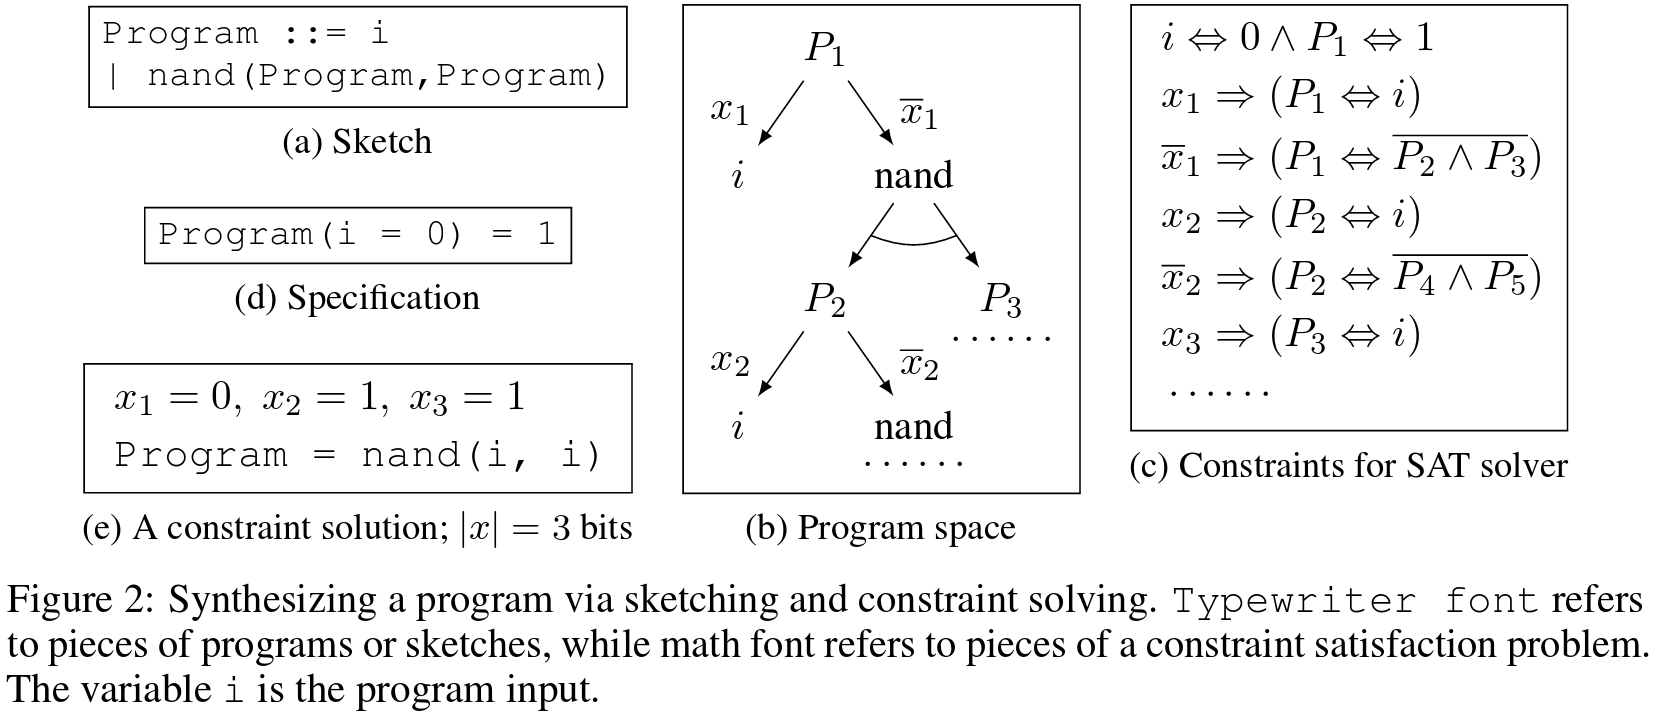
\includegraphics[width=45cm]{background.png}
  \end{block}

  \begin{block}{Sampling by Random XOR Constraints}

 \hspace{5.5cm}\begin{tikzpicture}\centering
%      \node[] at (0,0){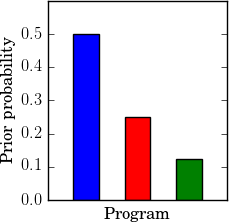
\includegraphics[width = 15cm]{notsliced.png}};
%      \node[] at (-15,0){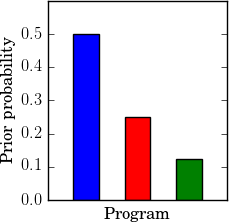
\includegraphics[width = 15cm]{notsliced.png}};
      \node[] at (0,0){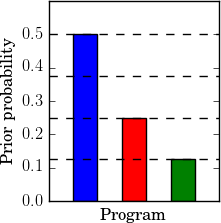
\includegraphics[width = 15cm]{sliced.png}};
      \draw [-,ultra thick]  (9,0) -- (13,0) -- (13,-1) -- (15,0.5) -- (13,2) -- (13,1) -- (9,1) -- (9,0);
      \node at (20,7) {Embedding $E$};
      \draw[ultra thick] (20,0) ellipse (3cm and 6cm);
      \draw[fill,blue] (21.3,3) circle [radius = 0.7];
      \draw[fill,blue] (21,-3) circle [radius = 0.7];
      \draw[fill,blue] (19,3.9) circle [radius = 0.7];
      \draw[fill,blue] (18.5,0.7) circle [radius = 0.7];
      \draw[fill,red] (22,1) circle [radius = 0.7];
      \draw[fill,red] (19,-3.5) circle [radius = 0.7];
      \draw[fill,green] (20.2,-0.3) circle [radius = 0.7];
      %      \node[] at (20,0){
\includegraphics[width = 8cm]{embedded.png}};
      
      \end{tikzpicture}
    
% Embed program space in a set $E$ so that sampling uniformly from $E$ draws from the posterior.
 Sample approximately uniformly from $E$ by fixing the parity of random sums (XOR's) of SAT variables.
 Main idea in Ermon et al. 2013.

\textbf{Definition: Tilt.} The \emph{tilt} of $p(\cdot)$ is $\frac{\max_x p(x)}{\min_x p(x)}$.
 
 \textbf{A problem.} Very inefficient if  the posterior $p(x)$ is highly tilted. \theSystem{} approximates $p(x)$ by a low tilt distribution $q(x)$. Rejection sampling corrects this distortion: $A(x)$ is acceptance probability.

\vspace{0.9cm}
  \begin{tabular}{cl}
    \begin{tabular}{c}
      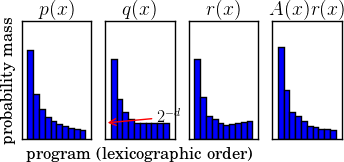
\includegraphics[width=25cm]{cartoon_small.png} 
    \end{tabular}&
    \begin{tabular}{l}
      \parbox{15cm}{\emph{Summary}: Approximate $p(x)$ by $q(x)$, embed in $E$, approximately uniform samples of $E$ give $r(x)$, distribution of samples is $\propto A(x)r(x)$}
      \end{tabular}
    \end{tabular}

  \end{block}

  \begin{block}{Theoretical guarantees}
    \theSystem{} takes two real-valued parameters, $\gamma$ and $\Delta$.

    \vspace{1cm}
    
    \textbf{Proposition 1: Distribution of samples is close in KL to the true posterior.}
    Write $Ar(x)$ to mean the distribution of the samples. Then $\text{KL}(p||Ar)<\log \left( 1 + \frac{1 + 2^{ - \gamma}}{1 + 2^\Delta}\right)$.

        \vspace{1cm}

    \textbf{Proposition 2: Not too much work is needed to get a sample.}
    The expected number of calls to the solver per sample is bounded above by $\frac{1 + 2^\Delta}{(1 + 2^{ - \gamma})^{-1}(1 + 2^{ - \Delta})^{-1} - 2^{ - \Delta}}.$

  \end{block}

%----------------------------------------------------------------------------------------

\end{column} % End of column 2.1

\begin{column}{\onecolwid}\vspace{-.6in} % The second column within column 2 (column 2.2)

%----------------------------------------------------------------------------------------
%	METHODS
%----------------------------------------------------------------------------------------

\begin{block}{Domain: Learning text edit scripts}

  \textbf{Programming By Example}: Learn a string editing program from a few examples. Systems like this ship in Microsoft Excel. 

  \vspace{1cm}
  
  \begin{tabular}{lr}\toprule
  \textbf{Examples} & \textbf{A program}\\\midrule
\\\begin{tabular}{l|r}
  Input & Output \\\hline
don steve g.&dsg\\
Kevin Jason Mat&KJM\\
Jose Larry S&JLS\\
Arthur Joe Juan&AJJ\\
Raymond F. Timothy &RFT
\end{tabular}&
\begin{tabular}{l}
  \parbox{25cm}{  \texttt{SubStr(0,1)+}
    \\\texttt{SubStr(Pos(' ','',0),Pos(' ','',0))+}
    \\\texttt{SubStr(Pos(' ','',-1),Pos(' ','',1))} }
\end{tabular}
\\\\
\hspace{3cm}\begin{tabular}{l|r}Input & Output \\\hline
12/31/13&12.31\\
1/23/2009&1.23\\
4/12/2023&4.12\\
6/23/15&6.23\\
7/15/2015&7.15
\end{tabular}&
\begin{tabular}{l}
  \hspace{2cm}\parbox{25cm}{  \texttt{SubStr(0,Pos('','/',0))+} \\
    \texttt{Constant('.')+}
    \\\texttt{SubStr(Pos('/','',0),Pos('','/',-1))}}
\end{tabular}

\\\\\bottomrule
  \end{tabular}

\vspace{1cm} \textbf{Key problem}: PBE systems target end-users who are unwilling to provide more than one or a few examples, leaving the intended behavior highly ambiguous. Model this ambiguity using sampling.
\end{block}

\begin{block}{Sketching a Program Space}
\centering\BUseVerbatim[fontfamily=courier]{TextSketch}
\end{block}

\begin{block}{Learning from very few examples}
\begin{figure}[h]\centering
  \begin{minipage}{0.45\textwidth}\centering
    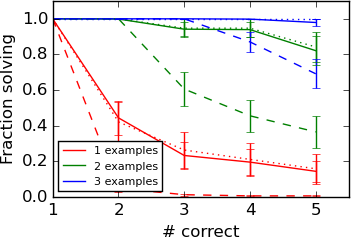
\includegraphics[width=\textwidth]{smallFractionSolving.png}
  \caption{Results averaged across 19 problems. Solid: \theSystem{} . Dashed: enumerating 100 programs. Dotted: MDL.}\label{flashPerformance}        \end{minipage}%
\hspace{0.025\textwidth}\begin{minipage}{0.45\textwidth}\centering
    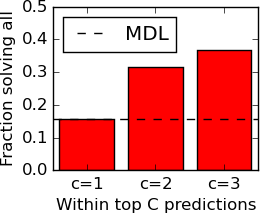
\includegraphics[width=0.7\textwidth]{small_mdl.png}
    \caption{MDL learner vs \theSystem{} on one-shot learning. Predictions marginalize out the program.}\label{mdl}
  \end{minipage}
\end{figure}

%\textbf{Multiple explanations aids one-shot learning.} After a single example, the shortest program is probably not correct -- but one of the top sampled \emph{behaviors} (marginalizing over the program) might be.

\textbf{Good performance needs tilt correction.} w/o low-tilt approximation, get no samples for any of these problems after an hour, vs $\approx 1$ minute w/ \theSystem



\end{block}

%% \begin{block}{The Cost of Sampling}
%%   Amortized cost of 100 samples from \theSystem :
  
%%   \vspace{1cm}

%%   \hspace{9cm}\vspace{1cm}    \begin{tabular}{lll}\toprule
%%      1 example\hspace{0.9cm}      &  2 examples\hspace{0.9cm}          &     3 examples\\\midrule
%% $84 \pm 3$ sec &$21 \pm 1$ sec & $49\pm 3$ sec
%% \end{tabular}

%% \textbf{Good performance needs tilt correction.} w/o low-tilt approximation, get no samples for any of these problems after an hour!

%% \textbf{Can closely approximate posterior with little overhead.}

%% %\vspace{-2.5cm}
%% \begin{tabular}{cl}
%%   \begin{tabular}{c}
%%     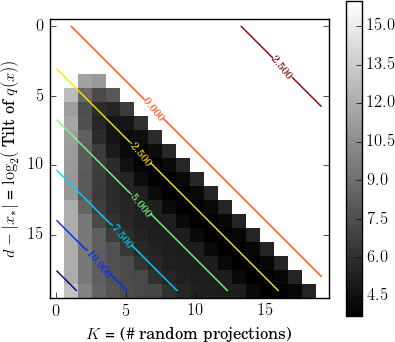
\includegraphics[width=25cm]{trim-trade-off.png}
%%     \end{tabular}&
%%   \begin{tabular}{l}
%%     \parbox{15cm}{Accuracy (colored contours) vs Performance (monochrome cells) trade-off; upper bounds plotted. Performance measured in expected solver invocations; accuracy measured in log KL divergence.}
%%     \end{tabular}
%% \end{tabular}
%% %\end{figure}

%%   \end{block}
%----------------------------------------------------------------------------------------

\end{column} % End of column 2.2

\end{columns} % End of the split of column 2 - any content after this will now take up 2 columns width


%----------------------------------------------------------------------------------------

\begin{columns}[t,totalwidth=\twocolwid] % Split up the two columns wide column again

 % End of column 2.1

\begin{column}{\onecolwid} % The second column within column 2 (column 2.2)

%----------------------------------------------------------------------------------------
%	RESULTS
%----------------------------------------------------------------------------------------


%----------------------------------------------------------------------------------------

\end{column} % End of column 2.2

\end{columns} % End of the split of column 2

\end{column} % End of the second column

\begin{column}{\sepwid}\end{column} % Empty spacer column

\begin{column}{\onecolwid} % The third column

%----------------------------------------------------------------------------------------
%	CONCLUSION
%----------------------------------------------------------------------------------------

  \begin{block}{Domain: List Manipulation}
    \textbf{Computer Aided Programming}: Synthesize source code consistent with a specification.
    We tackle these problems:
    \begin{itemize}
    \item \textbf{Sort}: synthesize quicksort
    \item \textbf{Reverse}: recursively reverse a list
    \item \textbf{Count}: count occurrences of list head in list tail
    \end{itemize}
    Multiple implementations might satisfy the spec, especially if the specs are examples.
    Model the ambiguity by sampling plausible implementations.

  \end{block}

  \begin{block}{Sketching a Program Space}
    \centering\BUseVerbatim[fontfamily=courier]{ListSketch}
  \end{block}

%----------------------------------------------------------------------------------------
%	ADDITIONAL INFORMATION
%----------------------------------------------------------------------------------------

\begin{block}{Learner Generalizes to Longer Sequences}
  Trained to sort, reverse, or count on lists of length $\leq 3$; tested on lists of length $\leq 14$.
  
\hspace{5cm}    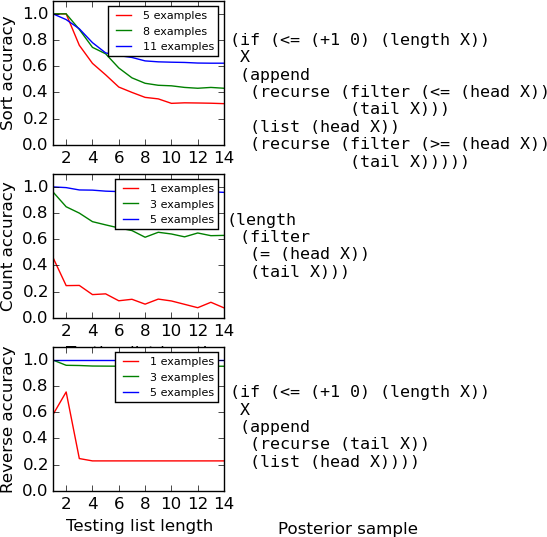
\includegraphics[width=33cm]{tinyList.png}

    \textbf{Sampling aids generalization.} Even if the most likely program has a bug, the posterior puts enough mass on correct programs that the ensemble of samples acts as a probabilistic algorithm with a high probability of succeeding.
    
\end{block}

%----------------------------------------------------------------------------------------
%	REFERENCES
%----------------------------------------------------------------------------------------

\setbeamercolor{block title}{fg=red,bg=white} % Change the block title color
%% \begin{block}{References}

%%   %\nocite{*} % Insert publications even if they are not cited in the poster
%%   \renewcommand{\refname}{\vspace{-0.8em}}
%%           \bibliographystyle{plain}
%%           \bibliography{main}
%% %\small{\bibliographystyle{plain}
%% %\bibliography{main}}

%% \end{block}

%----------------------------------------------------------------------------------------
%	ACKNOWLEDGEMENTS
%----------------------------------------------------------------------------------------

\setbeamercolor{block title}{fg=red,bg=white} % Change the block title color

%% \begin{block}{Acknowledgements}

%% \small{\rmfamily{We are grateful for feedback from Adam Smith, Kuldeep Meel, and our anonymous reviewers.
%% Work supported by AFOSR award FA9550-16-1-0012.}} \\

%% \end{block}

%----------------------------------------------------------------------------------------
%	CONTACT INFORMATION
%----------------------------------------------------------------------------------------


%----------------------------------------------------------------------------------------

\end{column} % End of the third column

\end{columns} % End of all the columns in the poster

\end{frame} % End of the enclosing frame

\end{document}

